\documentclass[a4paper,14pt]{extarticle}
\usepackage{../../tex-shared/report-layout}

\renewcommand{\mylabnumber}{6}
\renewcommand{\mylabtitle}{Исследование способов профилирования программного обеспечения}
\renewcommand{\mysubject}{Тестирование ПО}
\renewcommand{\mylecturer}{Тлуховская Н.П.}

\begin{document}
\begin{titlepage}
    
    \thispagestyle{empty}
    
    \begin{center}
        
        Министерство науки и Высшего образования Российской Федерации \\
        Севастопольский государственный университет \\
        Кафедра ИС
        
        \vfill

        Отчет \\
        по лабораторной работе №\mylabnumber \\
        \enquote{\mylabtitle} \\
        по дисциплине \\
        \enquote{\MakeTextUppercase{\mysubject}}

    \end{center}

    \vspace{1cm}

    \noindent\hspace{7.5cm} Выполнил студент группы ИС/б-17-2-о \\
    \null\hspace{7.5cm} Горбенко К. Н. \\
    \null\hspace{7.5cm} Проверил \\
    \null\hspace{7.5cm} \mylecturer

    \vfill

    \begin{center}
        Севастополь \\
        \the\year{}
    \end{center}

\end{titlepage}
\section{Цель работы}
Исследовать критические по времени выполнения участки программного
кода и возможности их устранения. Приобрести практические навыки анализа
программ с помощью профайлера EQATECProfiler.

\section{Порядок выполнения работы}
\begin{enumerate}
    \item Разработать программу на основе библиотеки классов, реализованной
    и протестированной в предыдущей работе. Программа должна как можно более
    полно использовать функциональность класса. При необходимости для
    наглядности профилирования в методы класса следует искусственно внести
    задержку выполнения.
    \item Выполнить профилирование разработанной программы, выявить
    функции, на выполнение которых тратится наибольшее время.
    \item Модифицировать программу с целью оптимизации времени
    выполнения.
    \item Выполнить повторное профилирование программы, сравнить новые
    результаты и полученные ранее, сделать выводы.
\end{enumerate}

\section{Ход работы}
Для тестирования напишем следующую программу:
\begin{lstlisting}
public static void Main(string[] args)
{
    var matrix = CreateMatrix();
    var sumsOfPositiveElementsInColumns = MatrixOperations.GetSumsOfPositiveElementsInColumns(matrix);

    foreach (var item in sumsOfPositiveElementsInColumns)
    {
        Console.WriteLine($"{item} ");
    }
    return;
}

private static int[,] CreateMatrix()
{
    var random = new Random();
    var matrix = new int[10000, 10000];

    for (var i = 0; i < 10000; i++)
    {
        for (var j = 0; j < 10000; j++)
        {
            matrix[i, j] = Enumerable.Range(0, random.Next(1, 1000)).Select(x => random.Next(int.MinValue, int.MaxValue))
                                     .ToArray()
                                     .Last();
        }
    }

    return matrix;
}
\end{lstlisting}

В данной программе создается массив 10000x10000 целочисленных элементов. Каждый элемент
создается путем взятия последнего элемента последовательности случайных чисел случайной
длины. Затем, для каждого столбца матрицы рассчитывается сумма положительных элементов.
В конце каждый элемент преобразовывается к строке, из каждой части склеивается одна строка
и выводится на экран.

Потенциально, наибольшее время может тратиться на создание массива, вычисление суммы столбцов,
преобразование элементов к строкам, запись большой строки в консоль. Запустим профилировщик:
\begin{figure}[H]
    \centering
    
\includegraphics[width=.8\linewidth]{before}
    \caption{Результаты профилирования программы}
    \label{fig:before}
\end{figure}

Время выполнения программы - 14,345 с. Из профилирования программы видно, что подавляющее большинство времени программы заняли
вызовы метода ToArray(). При вызове этого метода происходило копирование элементов в новый массив. Исправим это место:
\begin{lstlisting}
public static void Main(string[] args)
{
    var matrix = CreateMatrix();
    var sumsOfPositiveElementsInColumns = MatrixOperations.GetSumsOfPositiveElementsInColumns(matrix);

    foreach (var item in sumsOfPositiveElementsInColumns)
    {
        Console.WriteLine($"{item} ");
    }
    return;
}

private static int[,] CreateMatrix()
{
    var random = new Random();
    var matrix = new int[10000, 10000];

    for (var i = 0; i < 10000; i++)
    {
        for (var j = 0; j < 10000; j++)
        {
            matrix[i, j] = Enumerable.Range(0, random.Next(1, 1000)).Select(x => random.Next(int.MinValue, int.MaxValue))
                                     .Last();
        }
    }

    return matrix;
}
\end{lstlisting}

Снова запустим профилировщик:
\begin{figure}[H]
    \centering
    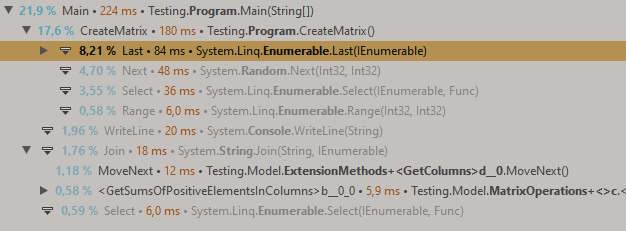
\includegraphics[width=.8\linewidth]{after}
    \caption{Результаты профилирования программы}
    \label{fig:after}
\end{figure}

Время выполнения программы сократилось 0.224 с.

\section*{Выводы}
В ходе лабораторной работы было выполнено профилирование программы. Оно позволяет
оценить время и память, затрачиваемые на вызов каждой функции. Это позволяет
определить места в программном коде, на которые стоит обратить внимание. Кроме того,
профилировщик позволяет построить граф вызовов функций. Это полезно например, для того,
чтобы определить частоту вызовов той или иной функции.
\end{document}